\documentclass[onecolumn, draftclsnofoot,10pt, compsoc]{IEEEtran}
\hbadness=1000 % suppress warnings
\usepackage{graphicx}
\usepackage{url}
\usepackage{setspace}
\usepackage{hyperref}
\usepackage{listings}
\usepackage{geometry}
\usepackage{caption}

\geometry{textheight=9.5in, textwidth=7in}

% 1. Fill in these details
\def \CapstoneTeamName{			}
\def \CapstoneTeamNumber{		69}
\def \GroupMemberOne{			Kin-Ho Lam}
\def \GroupMemberTwo{			Lucien Armand Tamdja Tamno}
\def \CapstoneProjectName{		Depth Sensing using Computer Vision and Lidar}
\def \CapstoneSponsorCompany{	Oregon State University}
\def \CapstoneSponsorPerson{	D. Kevin McGrath}


% 2. Uncomment the appropriate line below so that the document type works
\def \DocType{		%Problem Statement
	%Requirements Document
	%Technology Review
	%Design Document
	Winter Midterm Progress Report
}

\newcommand{\NameSigPair}[1]{\par
	\makebox[2.75in][r]{#1} \hfil 	\makebox[3.25in]{\makebox[2.25in]{\hrulefill} \hfill		\makebox[.75in]{\hrulefill}}
	\par\vspace{-12pt} \textit{\tiny\noindent
		\makebox[2.75in]{} \hfil		\makebox[3.25in]{\makebox[2.25in][r]{Signature} \hfill	\makebox[.75in][r]{Date}}}}
% 3. If the document is not to be signed, uncomment the RENEWcommand below
\renewcommand{\NameSigPair}[1]{#1}

%%%%%%%%%%%%%%%%%%%%%%%%%%%%%%%%%%%%%%%
\graphicspath{{images/}}
\begin{document}
	\begin{titlepage}
		\pagenumbering{gobble}
		\begin{singlespace}
			\centering
			
\includegraphics[height=4cm,natwidth=345,natheight=435]{images/osu_logo.png}
			\hfill 
			% 4. If you have a logo, use this includegraphics command to put it on the coversheet.
			%\includegraphics[height=4cm]{CompanyLogo}   
			\par\vspace{.2in}
			\centering
			\scshape{
				\huge Senior Design Capstone \DocType \par
				{\large\today}\par
				\vspace{.5in}
				\textbf{\Huge\CapstoneProjectName}\par
				\vfill
				{\large Prepared for}\par
				\Huge \CapstoneSponsorCompany\par
				\vspace{5pt}
				{\Large\NameSigPair{\CapstoneSponsorPerson}\par}
				{\large Prepared by }\par
				Group\CapstoneTeamNumber\par
				% 5. comment out the line below this one if you do not wish to name your team
				\CapstoneTeamName\par 
				\vspace{5pt}
				{\large
					\NameSigPair{\GroupMemberOne}\par
					\NameSigPair{\GroupMemberTwo}\par
				}
				\vspace{20pt}
			}
			\begin{abstract}  
 				Depth Sensing with Computer Vision and LIDAR proposes combining computer vision and LIDAR to create a reliable depth sensor.
				This document details its project member's progress toward a final design, and future milestones.
			\end{abstract}     
		\end{singlespace}
	\end{titlepage}
\section{Table of Contents}
\tableofcontents
\bibliographystyle{IEEEtran}
\bibliography{ref}
\clearpage

\begin{singlespace}
	\section{Definitions}
		\subsection{IR}\label{def:IR}
		IR refers to the infrared light spectrum.

		\subsection{IR Depth Sensor}\label{def:depthsensor}
		A device that calculates distances by emitting infrared patterns. 
		
		\subsection{LIDAR}\label{def:lidar}
		Light Detection And Ranging - A method that uses lasers to measure distance
		
		\subsection{Microsoft Kinect}\label{def:kinect}
		A product that uses an IR Depth sensor to measure distances.
		
		\subsection{Logitech Brio Webcam}\label{def:brio}
		The webcam model this project shall be using.
		
		\subsection{RPLidar A1}\label{def:rplidar}
		A low-cost LIDAR unit that this project shall be using.
		
		\subsection{Computer Vision }\label{def:vision}
		The methods for acquiring, processing, analyzing, and classifying digital images and extracting information.
		
		\subsection{GUI}\label{def:gui}
		GUI: Graphical User Interface
		
		\subsection{Videocapture}\label{def:videocapture}
		videocapture: Stream of subsequent images
		
		
		
	\section{Project Purpose}
		Commercial infrared-based depth sensors such as the model used in Microsoft's Kinect can quickly calculate distances in indoor scenarios.
		However, IR depth sensors can be confused by other infrared emitters such as other IR depth sensors or natural sunlight.
		For these reasons, IR depth sensors cannot be used in self-driving cars, outdoor robots, or any any device that requires high accuracy and reliable distance calculation.

		Depth Sensing with Computer Vision and LIDAR proposes combining the power of computer vision with the reliability of LIDAR technology.
		LIDAR uses a pulsing laser to measure relative distance.
		The LIDAR unit we're going to be using is called the RPLidar A1.
		We'll be combining this with a high-end Logitech Brio webcam.

	\section{Current State}

	\subsection{Kin-Ho Lam}
		\subsubsection{Proposed Design}
			The Logitech Brio webcam provides two-dimensional image but lacks depth perception.
			The RPLidar A1 LIDAR provides accurate depth measurement in a horizontal dimension but lacks vertical depth sensing.
			Combining the functionality of both devices to get accurate three-dimensional depth sensing presents a unique engineering challenge.
			This project proposes bridging the utility of both devices by securing them in stationary positions, then using software to combine their outputs.
			This involves using the RPLidar's library to get depth sensing information, and using computer vision to recognize objects.
			
			\begin{figure}[here]
				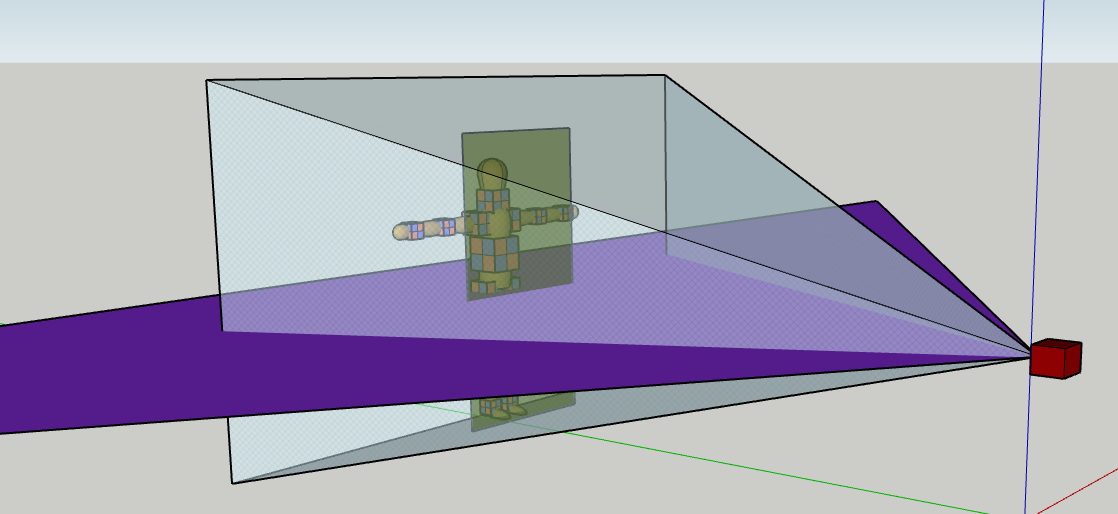
\includegraphics[scale=0.5]{different_dimensions.PNG}
				\captionof{figure}{Visualizing different dimensions measured by the RPLidar and Brio Webcam.}
				\label{dimensions}
			\end{figure}

			Figure \ref{dimensions} illustrates different dimensions measured by the RPLidar and Brio Webcam.
			The red cube represents the Logitech Brio webcam and RPLidar device secured in stationary positions.
			The flat purple triangle represents the RPLidar's horizontal range detection.
			The transparent green rectangle in front of the person represents the computer vision model recognizing that there is a person in-front of the sensor.
			The transparent teal pyramid represents the Brio webcam's field-of-view.
			
			\begin{figure}[here]
				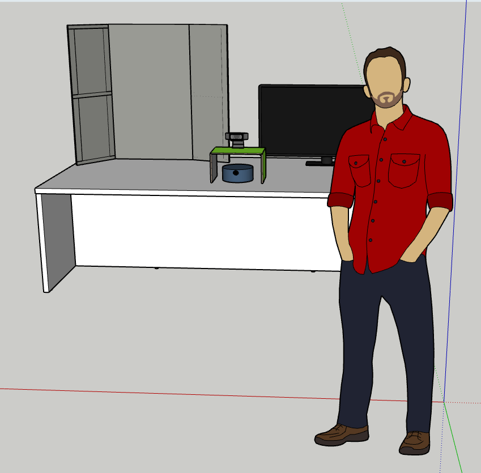
\includegraphics[scale=0.5]{expo.PNG}
				\captionof{figure}{Expo/final design concept}
				\label{expo}
			\end{figure}

			Figure \ref{expo} illustrates the project's final expo design.
			This render depicts the Brio webcam and RPLidar A1 in fixed positions.
			The software shall be capable of displaying the video output of the webcam with object distance information overlaid.
			The Brio webcam serves to provide subject identification and a point of reference in the vertical axis.
			The RPLidar A1 serves to provide distance measurement in the horizontal plane.
			As illustrated in Figure \ref{dimensions}, the horizontal range of the RPLidar A1 extends beyond the Brio webcam's field of view.
			This requires software adjustments such that the RPLidar A1's data is restricted to only collecting data within the camera's FOV.
			Fixing both devices in stationary positions simplifies this task.
			Once relevant distance information can be parsed, the software shall then use computer vision to recognize contiguous objects such as people.
			If a person is identified and the RPLidar A1 detects an object is within the camera's field of view, the software shall overlay distance 

			\begin{figure}[here]
				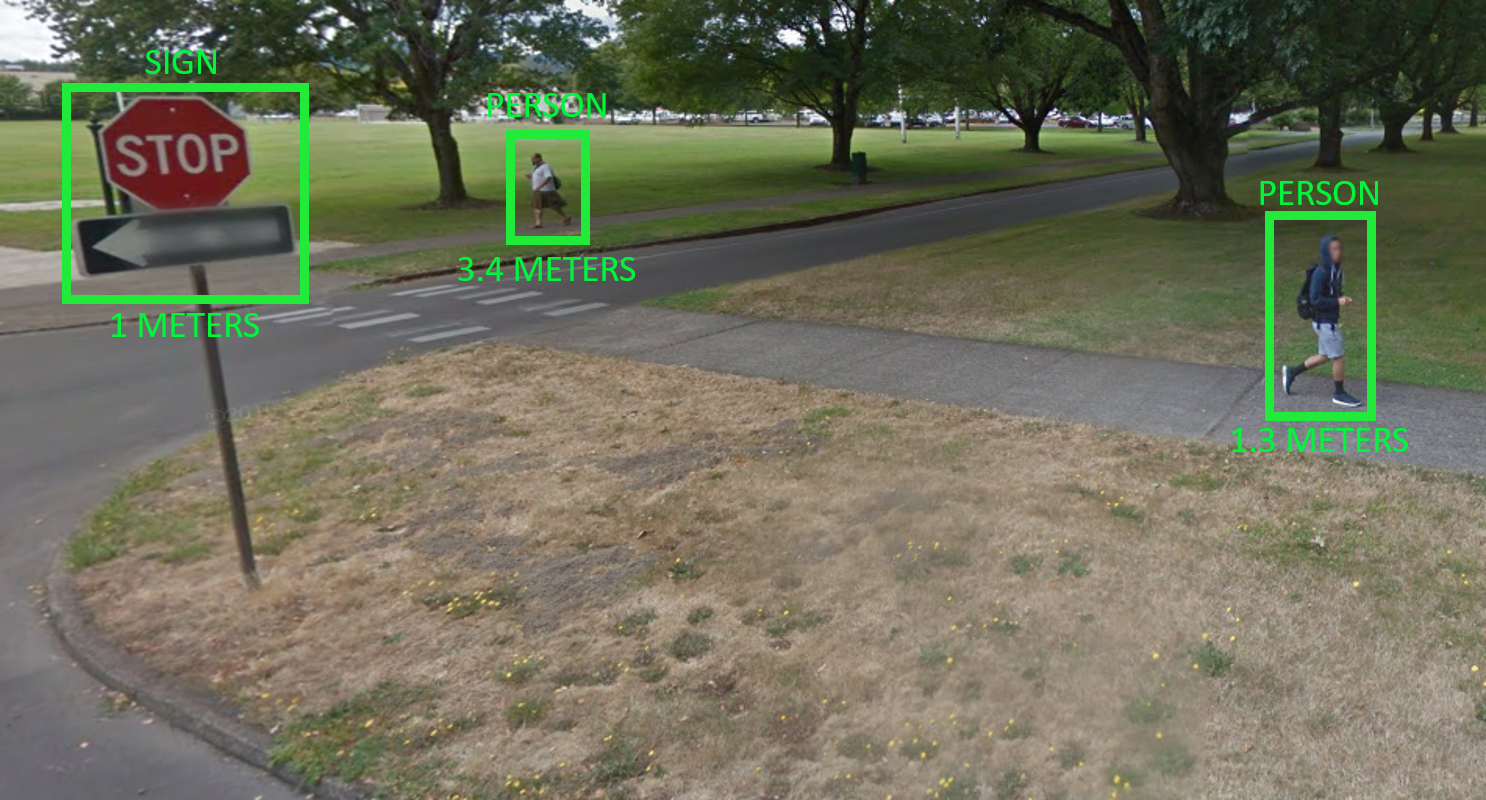
\includegraphics[scale=0.4]{overlay_design.png}
				\captionof{figure}{Distance overlay concept}
				\label{overlay}
			\end{figure}

		\subsubsection{Computer Vision}
			Figure \ref{svm} illustrates my current progress towards creating an accurate computer vision model.
			I am modifying a pre-trained SVM to recognize faces.
			The SVM can recognize faces in various lighting conditions even if the subject is wearing hats or glasses.
			This algorithm is not completely reliable or accurate, if the subject turns their face away from the camera or is looking off-center, the model will fail to recognize their face.
			This program is written in Python 3 and uses OpenCV 3.4.0. \cite{opencv}

			\begin{figure}[here]
				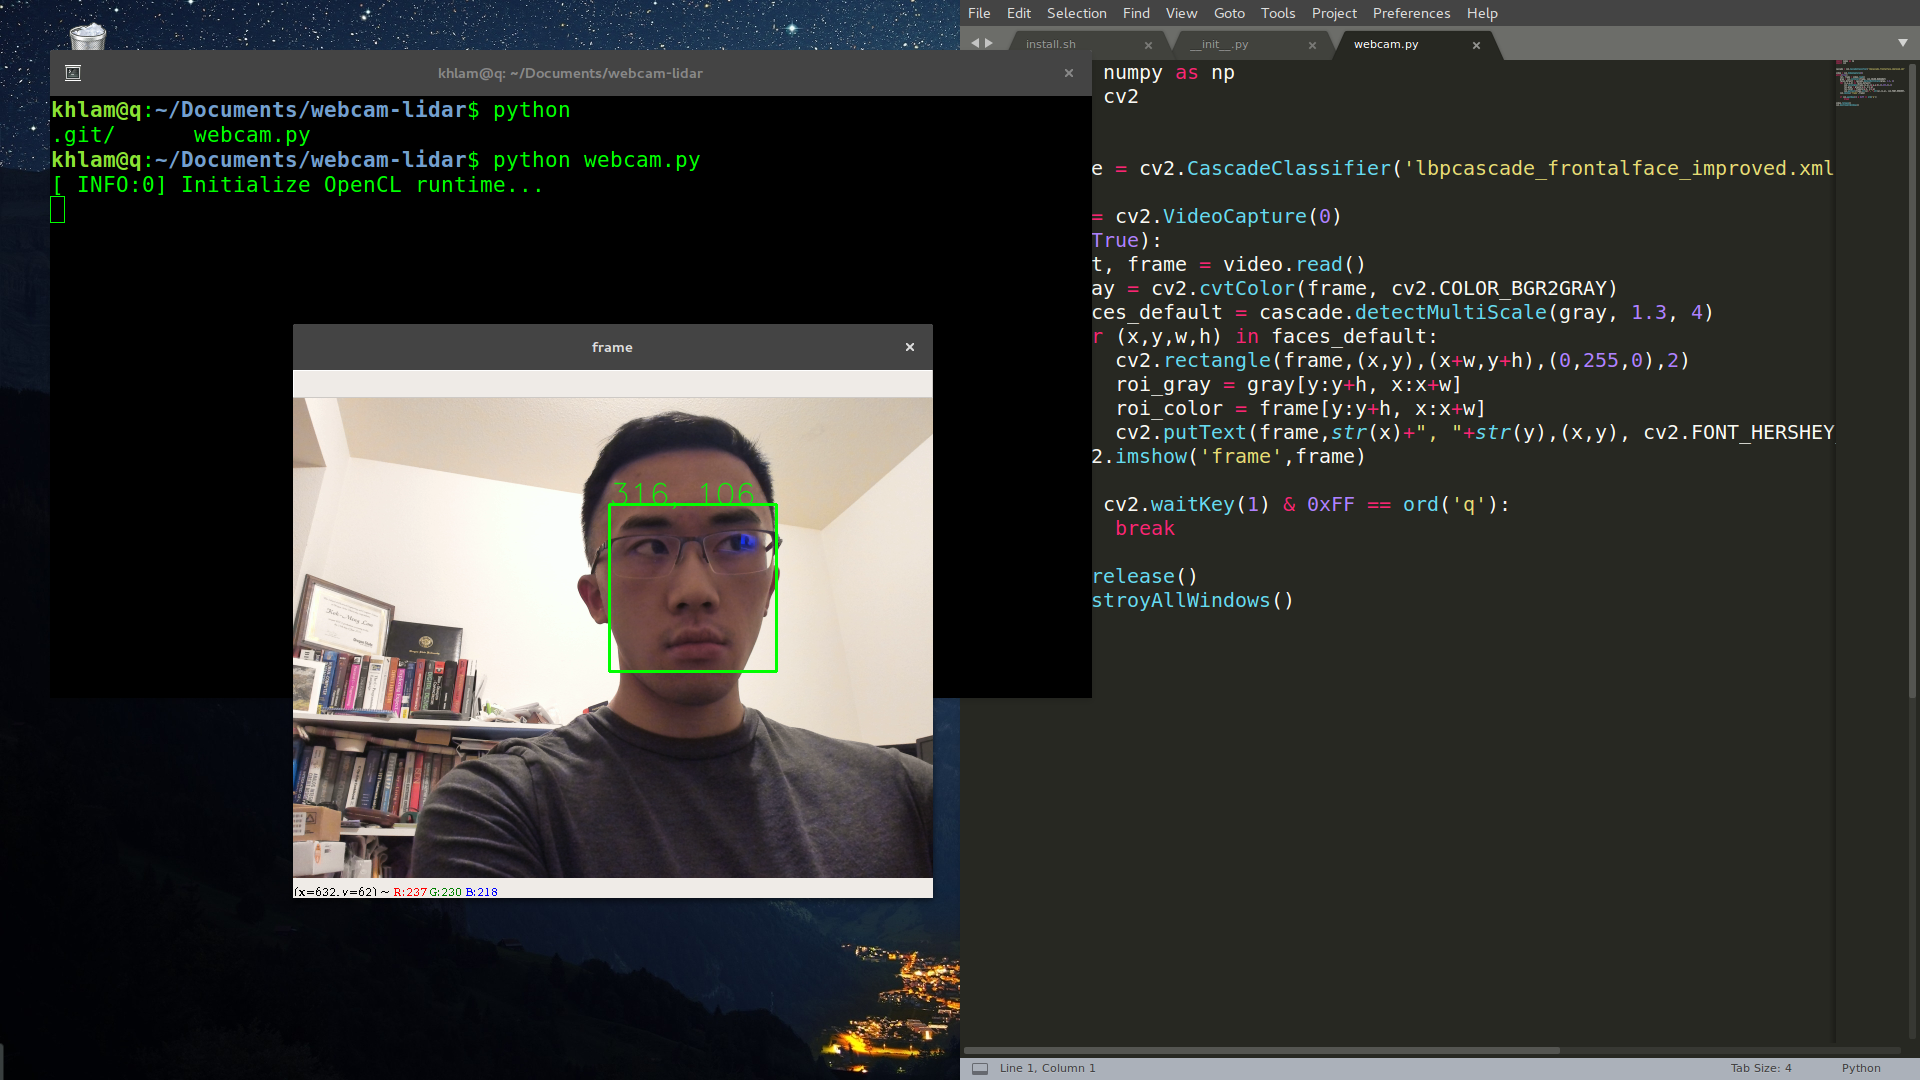
\includegraphics[scale=0.3]{lam_SVM_progess.png}
				\captionof{figure}{Face detection demonstration using a pre-trained SVM. The green box is recognized as a face.}
				\label{svm}
			\end{figure}

		\subsubsection{Future Milestones}
			I hope to expand the SVM's capabilities to recognize full or half bodies.
			I am exploring open-source algorithms to perform this task, and I am confident recognizing full or half bodies is possible.
			After my colleague Lucian completes his research into extracting depth sensing information from the RPLidar, I shall assist him in calibrating the software to only perform depth measurements within the webcam's field of view.


	\subsection{Lucien Armand Tamdja Tamno}
	
		\subsubsection{Introduction}
			This part of the process report primarily explain the various steps we took  to write the Graphical user Interface as well as the backend function that allows someone to get frames from an input stream video from a camera to store  images on a file. So,  In the following sections, we first define the purpose of the graphical interface built, and then, we extend the definition by showing how that GUI  was implemented, tools used to reach that implementation  and subsequently talk about one of the function that would be run when the interface is properly run. Finally, we conclude by mentioning problems encountered during the current progress. 
		
		\subsubsection{Purpose and goal of the GUI}	
			The GUI of this project is to primarily address its client needs and its existence is  to easily allow our client to enter information in a friendly way in order to get intended outcomes. Not only limited to be used by its client, the program can be exploited by anyone who is  either interested to use its results or to merely understand how the program works. The  interaction happening between a user and the program has to be friendly as possible and that is the goal of our GUI.

	However, if the GUI is used by anyone who can read between lines, that is doesn’t mean the interface alone does the whole job. In other words, we want to say that behind what the user sees there is other functions that are being run in order for the user to get what he or she will see on a screen.
	
		\subsubsection{ Python GUI and  Video capturing function}
			Tools used to build the GUI interface were first the current version of python package namely python 3.6 to which we combine with a GUI programming library  called the “ appJar “ [1] library. It  turns out this latter library only works well with the former python version due to certain common functionalities found in both, but also to note that the appJar was recently upgraded for the its users to get benefits of all advanced features it can offer like easy interaction with functions run on any  Windows, MacOS or Linux platform.  
So using this library, we were able to  display the following interface.

			\begin{figure}[here]
				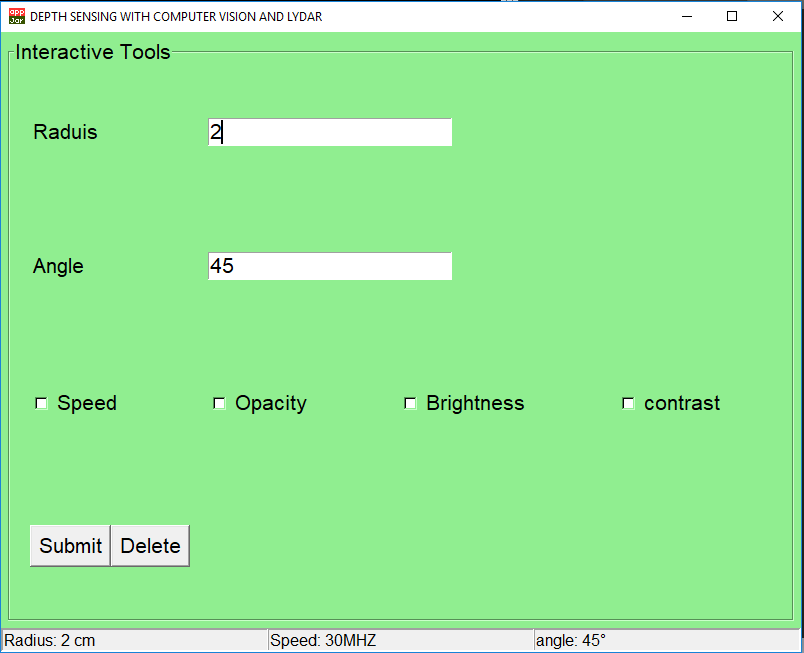
\includegraphics[scale=0.4, width=\textwidth]{userinterface.PNG}
				\captionof{figure}{sample  GUI for the depth sensing with computer vision and Lidar.}
				\label{gui}
			\end{figure}
			
		\subsubsection{ Python GUI }
				
			
			Though  we have to admit the fact that this above interface is not the final user interface for this project and also does not have enough documentation for us to write certain required functions like the function that should allow a user to click on the “submit button” and gets the program  perform certain  backend task like the video capturing of which we provide further details hereafter.
			
			\subsubsection{ Video-captured function  }
				The video capturing function processes an input stream of data to be outputted as  images  to in a given file. However to see this function at work, we needed several python libraries to come together.
		
		Therefore, the first  we did was to install the OpenCv library in windows environment to which we added another python library called numpy.   From these two libraries, we were able to perform basic tasks but more than that was still needed. The next step was to include to this package other tools  like the  “ glob” [2] library and some C++ functions namely the power and the square functions that we  imported from this website [3]. As a result,The following  snippet code script was written.

			\begin{figure}[here]
				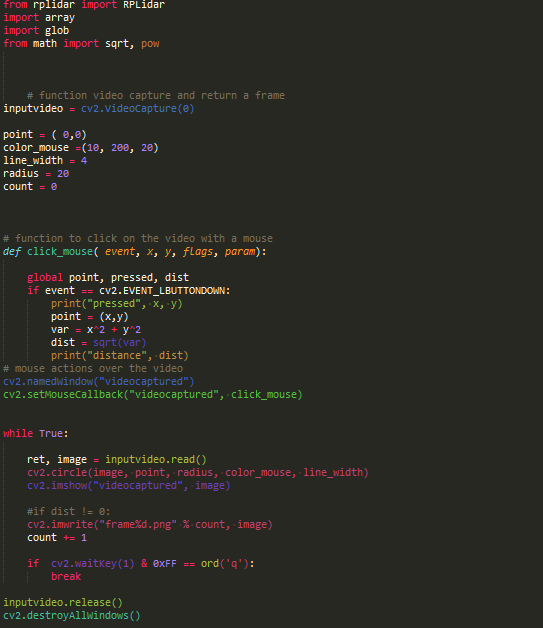
\includegraphics[scale=0.4, width=\textwidth]{videocapture.PNG}
				\captionof{figure}{ video-captured code.}
				\label{videocapture}
			\end{figure}
			
	In Spite of the current level of project progress but  to reach the final expected goal which is to overlay two images from two different sources ( camera and lidar device), we still have some work to do. Yet, even at this stage of project there is already barriers to hinder its good progress and  proper implementation. 
	\cite{guiprogramming}
	\cite{python}
	\cite{cplusplus}
		\section{Problems}
		This project and group was formed during Week 3. While the scale and purpose of this project is clear, a lot of work is necessary to construct an alpha-level demo. And among other problems, it still unclear what technique works, for us to run the RPLidar on Windows environment. Just because we want to test certains RPlidar functions on windows in order to use the full library in one end and in the other,our software should not be limited to any particular host environment ( Windows, MacOS or Linux ). Its  flexibility has to be experimented across platforms to make sure that wherever the software is used, it will provide the same outcome.

		
\end{singlespace}
\end{document}
